\documentclass[a4paper,openright,oneside]{thesis} %titlepage,openright,twoside,

%--------------------PREAMBLE----------------------------------------
\usepackage[utf8]{inputenc} %f ̧r Windows %direct gebruik van accenten
\usepackage[T1]{fontenc}
\usepackage[small,normal,bf,up]{caption}
\usepackage{eurosym,supertabular,multirow,tabularx} %,bigstrut,
\usepackage{geometry}
\usepackage{url} % om urls goed weer te geven in voetnoten
\usepackage[toc,page,title]{appendix}
\usepackage[multiple,flushmargin]{footmisc}
%\usepackage{cprotect} %gebruikt om verbatim in footnotes te zetten
\usepackage{hanging}% provides the \hangpara command
\usepackage{enumerate}
\usepackage[acronym,toc]{glossaries}  
\glsdisablehyper%
\makeglossaries%
\doublespacing%
\usepackage[babel]{csquotes}%



%--------------Layout van A4 document-----------------
\geometry{
  includeheadfoot,
  margin=2.5cm,
  hdivide={ ,19cm, }  
}

%------------------Footnotes--------------------------
\renewcommand{\footnotemargin}{1em}
% changes the above and sets the footnote mark just right of the left margin border.

\newcommand{\fn}[1]{\footnote{\hangpara{3em}{1} #1}}
% makes a new footnote command \fn{} with a hanging indent of 3em (hanging indent starts after the first line)

%------------Biblatex Optie 1---------------------------

%%\usepackage[backend=biber,style=authoryear-luh-ipw,isbn=false,url=false]{biblatex} %,style=historian ,citestyle=apa
%\usepackage[
%backend=biber,
%citestyle=authoryear-comp,
%bibstyle=authortitle,
%sorting=nyt,
%bibencoding=utf8,
%dashed=false,
%maxcitenames=1,
%isbn=false,
%url=false,
%babel=hyphen,
%hyperref=true,
%doi=false]
%{biblatex}


%--------Biblatex-------------------------------------

\DeclareNameAlias{sortname}{first-last}

\DeclareCiteCommand{\cite}[\mkbibbrackets]
  {\usebibmacro{prenote}}
  {\usebibmacro{citeindex}%
   \usebibmacro{cite}}
  {\multicitedelim}
  {\usebibmacro{postnote}}

\DeclareCiteCommand*{\cite}[\mkbibbrackets]
  {\usebibmacro{prenote}}
  {\usebibmacro{citeindex}%
   \usebibmacro{citeyear}}
  {\multicitedelim}
  {\usebibmacro{postnote}}


\newcounter{mymaxcitenames}
\AtBeginDocument{%
  \setcounter{mymaxcitenames}{\value{maxnames}}%
}

\renewbibmacro*{begentry}{%
  \printtext[brackets]{%
    \begingroup%
    \defcounter{maxnames}{\value{mymaxcitenames}}%
    \printnames{labelname}%
    \setunit{\nameyeardelim}%
    \usebibmacro{cite:labelyear+extrayear}%
    \endgroup%
    }%
  \quad% or \addspace
}

%--------END Biblatex-------------------------------------



%------------Biblatex Optie 2---------------------------

\PassOptionsToPackage{
        natbib=true,
        style=authoryear-comp,
        hyperref=true,
        backend=biber,
        maxbibnames=99,
        firstinits=true,
        uniquename=init,
        maxcitenames=2,
        parentracker=true,
        dashed=false,
        url=false,
        doi=false,
        isbn=false,
        eprint=false,
        backref=true,
            }   {biblatex}
\usepackage{biblatex}
\DeclareNameAlias{sortname}{last-first} 

% remove "in:" from articles. Thanks to Herbert.
\renewbibmacro{in:}{%
  \ifentrytype{article}{}{%
  \printtext{\bibstring{in}\intitlepunct}}}

% mit "month" and "language" from Bibliography
\AtEveryBibitem{%
  \clearfield{month}{}%
  \clearlist{language}{}%
  }

% some natbib backwards compatibility 
\let\citealp\cite
\let\cite\textcite

% increase vertical space between bibliography items.
\setlength\bibitemsep{0.5ex}
\setlength\bibnamesep{1.2ex}

% Comma before and after journal volume. Thanks to lockstep.
\renewbibmacro*{volume+number+eid}{%
  \setunit*{\addcomma\space}% NEW
  \printfield{volume}%
  \printfield{number}%
  \printfield{eid}}
  \DeclareFieldFormat[article]{number}{(#1)}% number of a journal

% Citation Hyperlinks (not just years), thanks to Audrey.
\makeatletter
\renewbibmacro*{cite}{% Based on cite bib macro from authoryear-comp.cbx
  \iffieldundef{shorthand}
    {\ifthenelse{\ifnameundef{labelname}\OR\iffieldundef{labelyear}}
       {\printtext[bibhyperref]{% Include labelname in hyperlink
          \DeclareFieldAlias{bibhyperref}{default}% Prevent nested hyperlinks
          \usebibmacro{cite:label}%
          \setunit{\addspace}%
          \usebibmacro{cite:labelyear+extrayear}}%
          \usebibmacro{cite:reinit}}
       {\iffieldequals{namehash}{\cbx@lasthash}
          {\ifthenelse{\iffieldequals{labelyear}{\cbx@lastyear}\AND
                       \(\value{multicitecount}=0\OR\iffieldundef{postnote}\)}
             {\setunit{\addcomma}%
              \usebibmacro{cite:extrayear}}
             {\setunit{\compcitedelim}%
              \usebibmacro{cite:labelyear+extrayear}%
              \savefield{labelyear}{\cbx@lastyear}}}
          {\printtext[bibhyperref]{% Include labelname in hyperlink
             \DeclareFieldAlias{bibhyperref}{default}% Prevent nested hyperlinks
             \printnames{labelname}%
             \setunit{\nameyeardelim}%
             \usebibmacro{cite:labelyear+extrayear}}%
             \savefield{namehash}{\cbx@lasthash}%
             \savefield{labelyear}{\cbx@lastyear}}}}
    {\usebibmacro{cite:shorthand}%
     \usebibmacro{cite:reinit}}%
  \setunit{\multicitedelim}}

\renewbibmacro*{textcite}{% Based on textcite bib macro from authoryear-comp.cbx
  \iffieldequals{namehash}{\cbx@lasthash}
    {\iffieldundef{shorthand}
       {\ifthenelse{\iffieldequals{labelyear}{\cbx@lastyear}\AND
                    \(\value{multicitecount}=0\OR\iffieldundef{postnote}\)}
          {\setunit{\addcomma}%
           \usebibmacro{cite:extrayear}}
          {\setunit{\compcitedelim}%
           \usebibmacro{cite:labelyear+extrayear}%
           \savefield{labelyear}{\cbx@lastyear}}}
       {\setunit{\compcitedelim}%
        \usebibmacro{cite:shorthand}%
        \global\undef\cbx@lastyear}}
    {\ifnameundef{labelname}
       {\printtext[bibhyperref]{% Include labelname in hyperlink
          \DeclareFieldAlias{bibhyperref}{default}% Prevent nested hyperlinks
          \iffieldundef{shorthand}
            {\usebibmacro{cite:label}%
             \setunit{%
               \global\booltrue{cbx:parens}%
               \addspace\bibopenparen}%
             \ifnumequal{\value{citecount}}{1}
               {\usebibmacro{prenote}}
               {}%
             \usebibmacro{cite:labelyear+extrayear}}
            {\usebibmacro{cite:shorthand}}%
          \ifthenelse{\iffieldundef{postnote}\AND
                      \(\value{multicitetotal}=0\AND\value{citetotal}=1\)}
            {\bibcloseparen% Include closing parenthesis in hyperlink
             \global\boolfalse{cbx:parens}}
            {}}}
       {\printtext[bibhyperref]{% Include labelname in hyperlink
          \DeclareFieldAlias{bibhyperref}{default}% Prevent nested hyperlinks
          \printnames{labelname}%
          \setunit{%
            \global\booltrue{cbx:parens}%
            \addspace\bibopenparen}%
          \ifnumequal{\value{citecount}}{1}
            {\usebibmacro{prenote}}
            {}%
          \iffieldundef{shorthand}
            {\iffieldundef{labelyear}
               {\usebibmacro{cite:label}}
               {\usebibmacro{cite:labelyear+extrayear}}%
             \savefield{labelyear}{\cbx@lastyear}}
            {\usebibmacro{cite:shorthand}%
             \global\undef\cbx@lastyear}%
          \ifthenelse{\iffieldundef{postnote}\AND
                      \(\value{multicitetotal}=0\AND\value{citetotal}=1\)}
            {\bibcloseparen% Include closing parenthesis in hyperlink
             \global\boolfalse{cbx:parens}}
            {}}%
          \savefield{namehash}{\cbx@lasthash}}}%
  \setunit{%
    \ifbool{cbx:parens}
      {\bibcloseparen\global\boolfalse{cbx:parens}}
      {}%
    \multicitedelim}}

\makeatother

% Backrefs "cited" instead of "cit"
\DefineBibliographyStrings{english}{%
backrefpage={cited on p\adddot},
backrefpages={cited on pp\adddot}
}



%------------------ FONT ----------------------------------------

% ALTERNATIVE
%\usepackage{lmodern}
%\usepackage[urw-garamond]{mathdesign}
%\usepackage[math]{iwona}
%\usepackage[default]{lato}
%\usepackage{venturis2}
\usepackage[sf]{quattrocento}
%\usepackage{libertine}
%\usepackage[T1]{fontenc}

%------------------ END FONT ------------------

\linespread{1.5} %\setlength{\parskip}{\baselineskip}
\setlength{\headheight}{43,3pt}
\setlength{\voffset}{0pt}

\pagestyle{fancy}
\fancyhf{}     % clear header & footer
\fancyhead[C]{\small\sf\nouppercase{\leftmark}}
\fancyhead[L]{
\includegraphics[width=.19\textwidth]{ThesisFigs/uva_logo}} %links tu logo
%\fancyhead[R]{thepage} %rechts Abbott logo \includegraphics[width=.2\textwidth]{ThesisFigs/abbott}
%\fancyfoot[L]{\thepage}
\fancyfoot[R]{\thepage}

\fancypagestyle{plain}{\fancyhf{}\fancyfoot[R]{\thepage}
\renewcommand{\headrulewidth}{0.4pt}
\renewcommand{\footrulewidth}{0.4pt}}

\renewcommand{\captionfont}{\small\textit}

\renewcommand{\headrule}{{\color{red}%
\hrule width\headwidth%
 height\headrulewidth \vskip-\headrulewidth}
 }
%\setlength{\footrulewidth}{\headrulewidth}
\renewcommand{\footrule}{{\color{blue}% 
  \vskip-\footruleskip\vskip-\footrulewidth%
\hrule width\headwidth height\footrulewidth\vskip\footruleskip}
}
\renewcommand{\chaptermark}[1]{\markboth{\textbf{\thechapter\ #1}}{}}
\renewcommand{\sectionmark}[1]{\markright{\thesection\ #1}{}}
\fancyheadoffset{0cm} % zorgt er voor dat de head en foot lijnen even breed zijn als de textbreedte


%--------title Opmaak------------------------

    \pdfinfo { /Title  (WTO LEadership)
               /Creator (TeX)
               /Producer (pdfTeX)
               /Author (Duco Wiertsema duco@wiertsema.net)
               /CreationDate (D:\today)  %format D:YYYYMMDDhhmmss
               /ModDate (D:20030815213532)
               /Subject (Writing a PhD thesis in LaTeX)
               /Keywords (PhD, Thesis)}
    \pdfcatalog { /PageMode (/UseOutlines)
                  /OpenAction (fitbh)  }


\title{Coevolution of the WTO and the and international business}
\subtitle{How do multiple embeddedness and coeevolution effect the decision making of MNE wrt the WTO}

  \author{\href{mailto:duco@wiertsema.net}{Duco Wiertsema}}
  \university{\href{http://www.uva.nl}{University of Amsterdam}}
% insert below the file name that contains the crest in-place of 'UnivShield'
  \crest{
\includegraphics[width=100mm]{uva_logo}}
%
\superA{}
\superB{}


% insert below the file name that contains the crest in-place of 'UnivShield'
% \crest{\IncludeGraphicsW{UnivShield}{40mm}{14 14 73 81}}
%
%\renewcommand{\submittedtext}{change the default text here if needed}
\degree{Master of Science in Business Studies}
\degreedate{June 2013}

% turn of those nasty overfull and underfull hboxes
\hbadness=10000
\hfuzz=40pt




%----------einde titel opmaak-------------------
%\floatplacement{table}{htbp} \floatplacement{figure}{htbp}
%\floatstyle{plaintop} \restylefloat{table}
%\renewcommand{\vec}{\boldsymbol}
%\newcommand{\unit}[1]{\ \mathrm{#1}}
%\newcommand{\srcinput}[2]{\noindent\framebox[\columnwidth]{\sc #2}{\scriptsize \verbatiminput{#1}}}
\setlength{\columnseprule}{\headrulewidth}
\setcounter{tocdepth}{2}


%% new commands \newcommand{name}[number of args][default argument values]{definition}


\newacronym{RBV}{RBV}{Resourced Based View}
\newacronym{IBV}{IBV}{Institutional Based View}
\newacronym{IB}{IB}{International business}
\newacronym{IP}{IP}{Intellectual Property}
\newacronym{MNE}{MNE}{Multinational Enterprises}
\newacronym{WTO}{WTO}{World Trade Organisation}
\newacronym{gatt}{GATT}{General Agreement on Tariffs and Trade}
\newacronym{IMF}{IMF}{International Monetary Fund}
\newacronym{WB}{World Bank}{World Bank}
\newacronym{FSA}{FSA}{Firm Specific Advantage}
\newacronym{BoD}{BoD}{Boards of Directors}
\newacronym{NGO}{NGO}{Non-Governmental Organisation}
\newcommand{\nego}{negotiations}
\newcommand{\wto}{\gls{WTO}}
\newcommand{\mne}{\gls{MNE}}
\newcommand{\ibv}{\gls{IBV}}
\newcommand{\rbv}{\gls{RBV}}
\newcommand{\ib}{\gls{IB}}
\newcommand{\fsa}{\gls{FSA}}
\newcommand{\iso}{isomorphism}
\newacronym{InBV}{Industry Based View}{Industry Based View}
\newacronym{NMA}{NMA}{Nederlande Mededingings Authoriteiten}
\newacronym{OFT}{OFT}{Office of Fairtrade}
\newacronym{CMA}{CMA}{Competition and Markets Authority}
\newacronym{ACM}{ACM}{Autoriteit Consument en Markt}

%---------Bibliography--------------------------------

\bibliography{Bibliography_papers.bib,Bibliography.bib}




%-------------Titel informatie----------------------
%Wordt in make title gegenereerd
%---------Begin Document----------------------------
\begin{document}
\cleardoublepage%
\maketitle%
%------------------Foreword-------------------------
\pagenumbering{roman}                         %
%\include{foreword/latex/Foreword}            %
%\addcontentsline{toc}{chapter}{Foreword}     %
%--------Abstract-----------------------------------
%\include{abstract/latex/abstract}
%\addcontentsline{toc}{chapter}{Abstract}
%%%%%%%%%%%%%%%%%%%%%%%%%%%%%%%%%%%%%%%%%%%%%%%
%------------Lists----------------------------------------------------------------

\renewcommand{\contentsname}{Table of Contents}  % Original name = Contents
%\begin{spacing}{1.2}  % Environment for 1.2 line spacing for contents and lists   |
\tableofcontents%
% \listoffigures \addcontentsline{toc}{chapter}{List of Figures}
 %\listoftables \addcontentsline{toc}{chapter}{List of Tables}
% \input{notations/latex/notations} \addcontentsline{toc}{chapter}{List Of Abbreviations}% and Symbols
\cleardoublepage%                                                                 |
%\end{spacing}%                                                                    |
%----------------------end--------------------------------------------------------

%%%%%%%%%%%%%%%%%%%%%%%%%%%%%%%%%%%%%%%%%%%%%%%
%   Arabic numbering after this               %
%%%%%%%%%%%%%%%%%%%%%%%%%%%%%%%%%%%%%%%%%%%%%%%
\newpage\thispagestyle{empty}\cleardoublepage%
\pagenumbering{arabic} \setcounter{page}{1}%

%------------Main Matter----------------------------


\chapter{Introduction}

\newacronym{WTO}{WTO}{World Trade Organisation}
\newacronym{gatt}{GATT}{General Agreement on Tariffs and Trade}
\newacronym{IMF}{IMF}{International Monetary Fund}
\newacronym{WB}{World Bank}{World Bank}

Trade has been as old as the Middle Paleolithic (300.000 to 30.000 years ago) and originated with the start of communication in prehistoric times. The first signs of trade have been discovered from around 150.000 years ago~\cite{Miller:2006}~\cite{Watson:2005}~\cite{Fernandez-Armesto:2003}~\cite{Mayell:2003}~\cite{Henahan:2002}. These first trades were in ochre, an earth pigment, used to dye fabrics. 
These trades were mainly in the form of bartered goods and services~\cite{OSullivan:2003} from each other before the
innovation of the modern day currency~\cite{Watson:2005}. \\ The innovation of money mend that barter~\footnote{according to \href{http://www.merriam-webster.com}{Merriam-Webster}: barter is 
\emph{to trade by exchanging one commodity for another}} was not longer a necessity to trade goods or services. With money medium common between the supplier and the demander became available. This facilitated a wider market and created the possibility of mercantilism~\cite{Heckscher:1936}. \\ That trade is an important aspect in our history, can be observed from the fact the silk route is still a well known aspect, although this route has  been out of commission in the way that was used. \\
\\
In some way money changed from a means to an objective. Amidst the financial turmoil that engulfed the world in 2012 and 2013, one may assume that ''\emph{Money makes the world go round}''. The quote has been around for some  time now, dating back to the musical \emph{Caberet} from the 1960s. \\ From a trade perspective money is still a means
As~\cite{Mises:2009} has defined: ``The function of money is to facilitate the business of the market by acting as a common medium of exchange``. By this line of thought the underlying motivation of money is the exchange of goods and  later services. 


After World War II much needed to change. The world had to come together. Hence 
two global albeit  of truly global organisations have 
For this purpose the \gls{IMF} and World Bank were founded in 
1944.
 

The  \gls{WTO} was established on January 1 1995. The \gls{WTO} came into existence after 
the \gls{gatt} had been dissolved into the \Gls{WTO}. 


%\chapter{Biography Pascal Lamy}

\subsubsection{Personal}
Pascal Lamy was born as  Pascal Lucien Fernand Lamy  on 8 April 1947 in Levallois Perret (Seine) France.
He is a son of Jacques Lamy and Denise Dujardin and has 
three children: Julien, David and Quentin.\\


\subsubsection{Education}
Lycée Carnot in Paris\\
    Graduate of the Ecole des Hautes Etudes Commerciales and
    the Institut d'Etudes Politiques in Paris (MBA)\\
    Postgraduate diploma in advanced legal studies
    University certificate in general literary studies
    
\subsubsection{Career}

\indent January 1973 to May 1975\\
Student at the Ecole Nationale d'Administration (“Léon Blum” contingent), graduated second in his year (economics section)\\

June 1975    \\
Posted to the Inspection Générale des Finances\\

1979\\
Secretary General of the “Mayoux Committee”\\
 Posted to the Direction du Trésor\\
 
1979 to 1981\\
Deputy Secretary General, then Secretary General of the Interministerial Committee for the Remodelling of Industrial Structures (CIASI) in the Treasury Department\\   

May 1981\\
 Technical Adviser, then Deputy Director (June 1982), Office of the Ministers for Economic and Financial Affairs (Mr Jacques Delors)\\  
 
April 1983 to July 1984\\
Deputy Director, Office of the Prime Minister (Mr Pierre Mauroy)\\

January 1985 to April 1994\\
Chef de Cabinet to the President of the Commission of the European Communities (Mr Jacques Delors)\\

May 1994\\
Crédit Lyonnais - Member of the Executive Committee\\

1999\\
Director General - Crédit Lyonnais\\ 

September 1999-2004\\
Commissioner for Trade at the European Commission -- Brussels\\  

Since Dec 2004\\
President of the Association ''Notre Europe`` \\
Associate Professor at Institut d’Etudes Politiques in Paris\\
      
\subsubsection{Military Service}

Lieutenant Commander (Navy)

  
\subsubsection{Decorations}

1999\\
Légion d'Honneur\\

1991\\
 Knight Commander's cross (Badge and Star) of the Order of Merit of the Federal Republic of Germany\\
      
1995\\
Commandor of the Order of Merit of Luxembourg\\
      
2000\\
 Officer of the Order of Merit of Gabon\\
      
2002\\
Doctor Honoris Causa of the University of Louvain (Belgium)\\
      
2003\\
Decorated in the Order of the Aztek Eagle (Mexico)\\
     
2004\\
Decorated in the Order of Merit of Chili\\
      

  
\subsubsection{Publications}
1979\\
    	Author with J.L. Bianco, of the report on Welfare Assistance for Children\\
      
1993\\
    Report on “Monde-Europe”; group presided by P. Lamy (XI Plan of the Commissariat Général au Plan)
      
2002\\
    “The Europe we want” (Plon) with Jean Pisani Ferry\\
      
2002\\
    “L’Europe en première ligne” (Seuil)\\
      
 2004\\
“La démocratie monde” (Seuil RDI)\\
      

\subsubsection{Sports}
Tennis, jogging and marathon
\chapter{Literature Review}



In an time of austerity and double dips in the economy, \gls{IB} is playing the game on different fields. Companies like Apple and Samsung are not only fighting for customers but also fighting in court over\gls{IP} as well. Next to this fight over \gls{IP} subsidies are at the forefront of the public debate as well. Boeing and Airbus have been fighting over subsidies for decades where on more than one occasion the \gls{WTO} has ruled on the validity of these subsidies. More recently solar panels have become a topic of tariffs between the European Union and China. \\

The field of play is governed by governments, trade blocks and the \gls{WTO} on the one hand and \gls{IB} on the other.
A multitude of forces are acting on this playing field and the different actors on this pitch have to cooperate. 
Different \gls{MNE} will cope differently with the challenges that are set by the institutions and the environment that they are operating in. That this environment is of importance is explained by \gls{IBV}~\cite{Kostova:1999,Meyer:2009,Wang:2012} 

\section{\glsdesc{IBV} in international Business}

\gls{IBV} has been a reaction on the theory of \gls{RBV} introduced by~\cite{Barney:1991}. The \gls{RBV} theory has gained a lot of support in the international business community. The aforementioned article has received more than 5000 citations
\footnote{according to Google Scholar
 %(http://scholar.google.nl/scholar?cites=3429746403909254791&as_sdt=2005&sciodt=0,5&hl=nl)
} 
since it has been published in 1991.\\ 

Where \gls{RBV} stated that a firms strategic advantage is depended on it's heterogeneous resources (a bundle of all assets, knowledge, and capabilities) which have to be
\begin{enumerate}[(a)]
\item must be valuable, in the sense that it exploit opportunities and/or neutralises threats in a firm’s environment
\item must be rare among a firm’s current and potential competition, 
\item must be imperfectly imitable
\item  there cannot be strategically equivalent substitutes for this resource that are valuable but neither rare or imperfectly imitable 
\end{enumerate} 
This concept is also known under the acronym VRIN.\\

In contrast to~\gls{RBV}, which in introspective in nature,~\gls{IBV} is extrospective.~\ibv~takes into 
account not only strategic choices driven by industry conditions and firm\-specific resources that 
traditional strategy research emphasises (\cite{Porter:1980},~\cite{Barney:1991}), but are also a 
reflection of the formal and informal constraints of a particular institutional framework that decision
makers confront (\cite{Oliver:1997,Scott:1995}). These institutions are influencing the decision making process in \gls{IB}.  The dynamic that takes place is depicted in picture \ref{fig:ibv}. 

\begin{figure}[htbp!] 
	\centering
	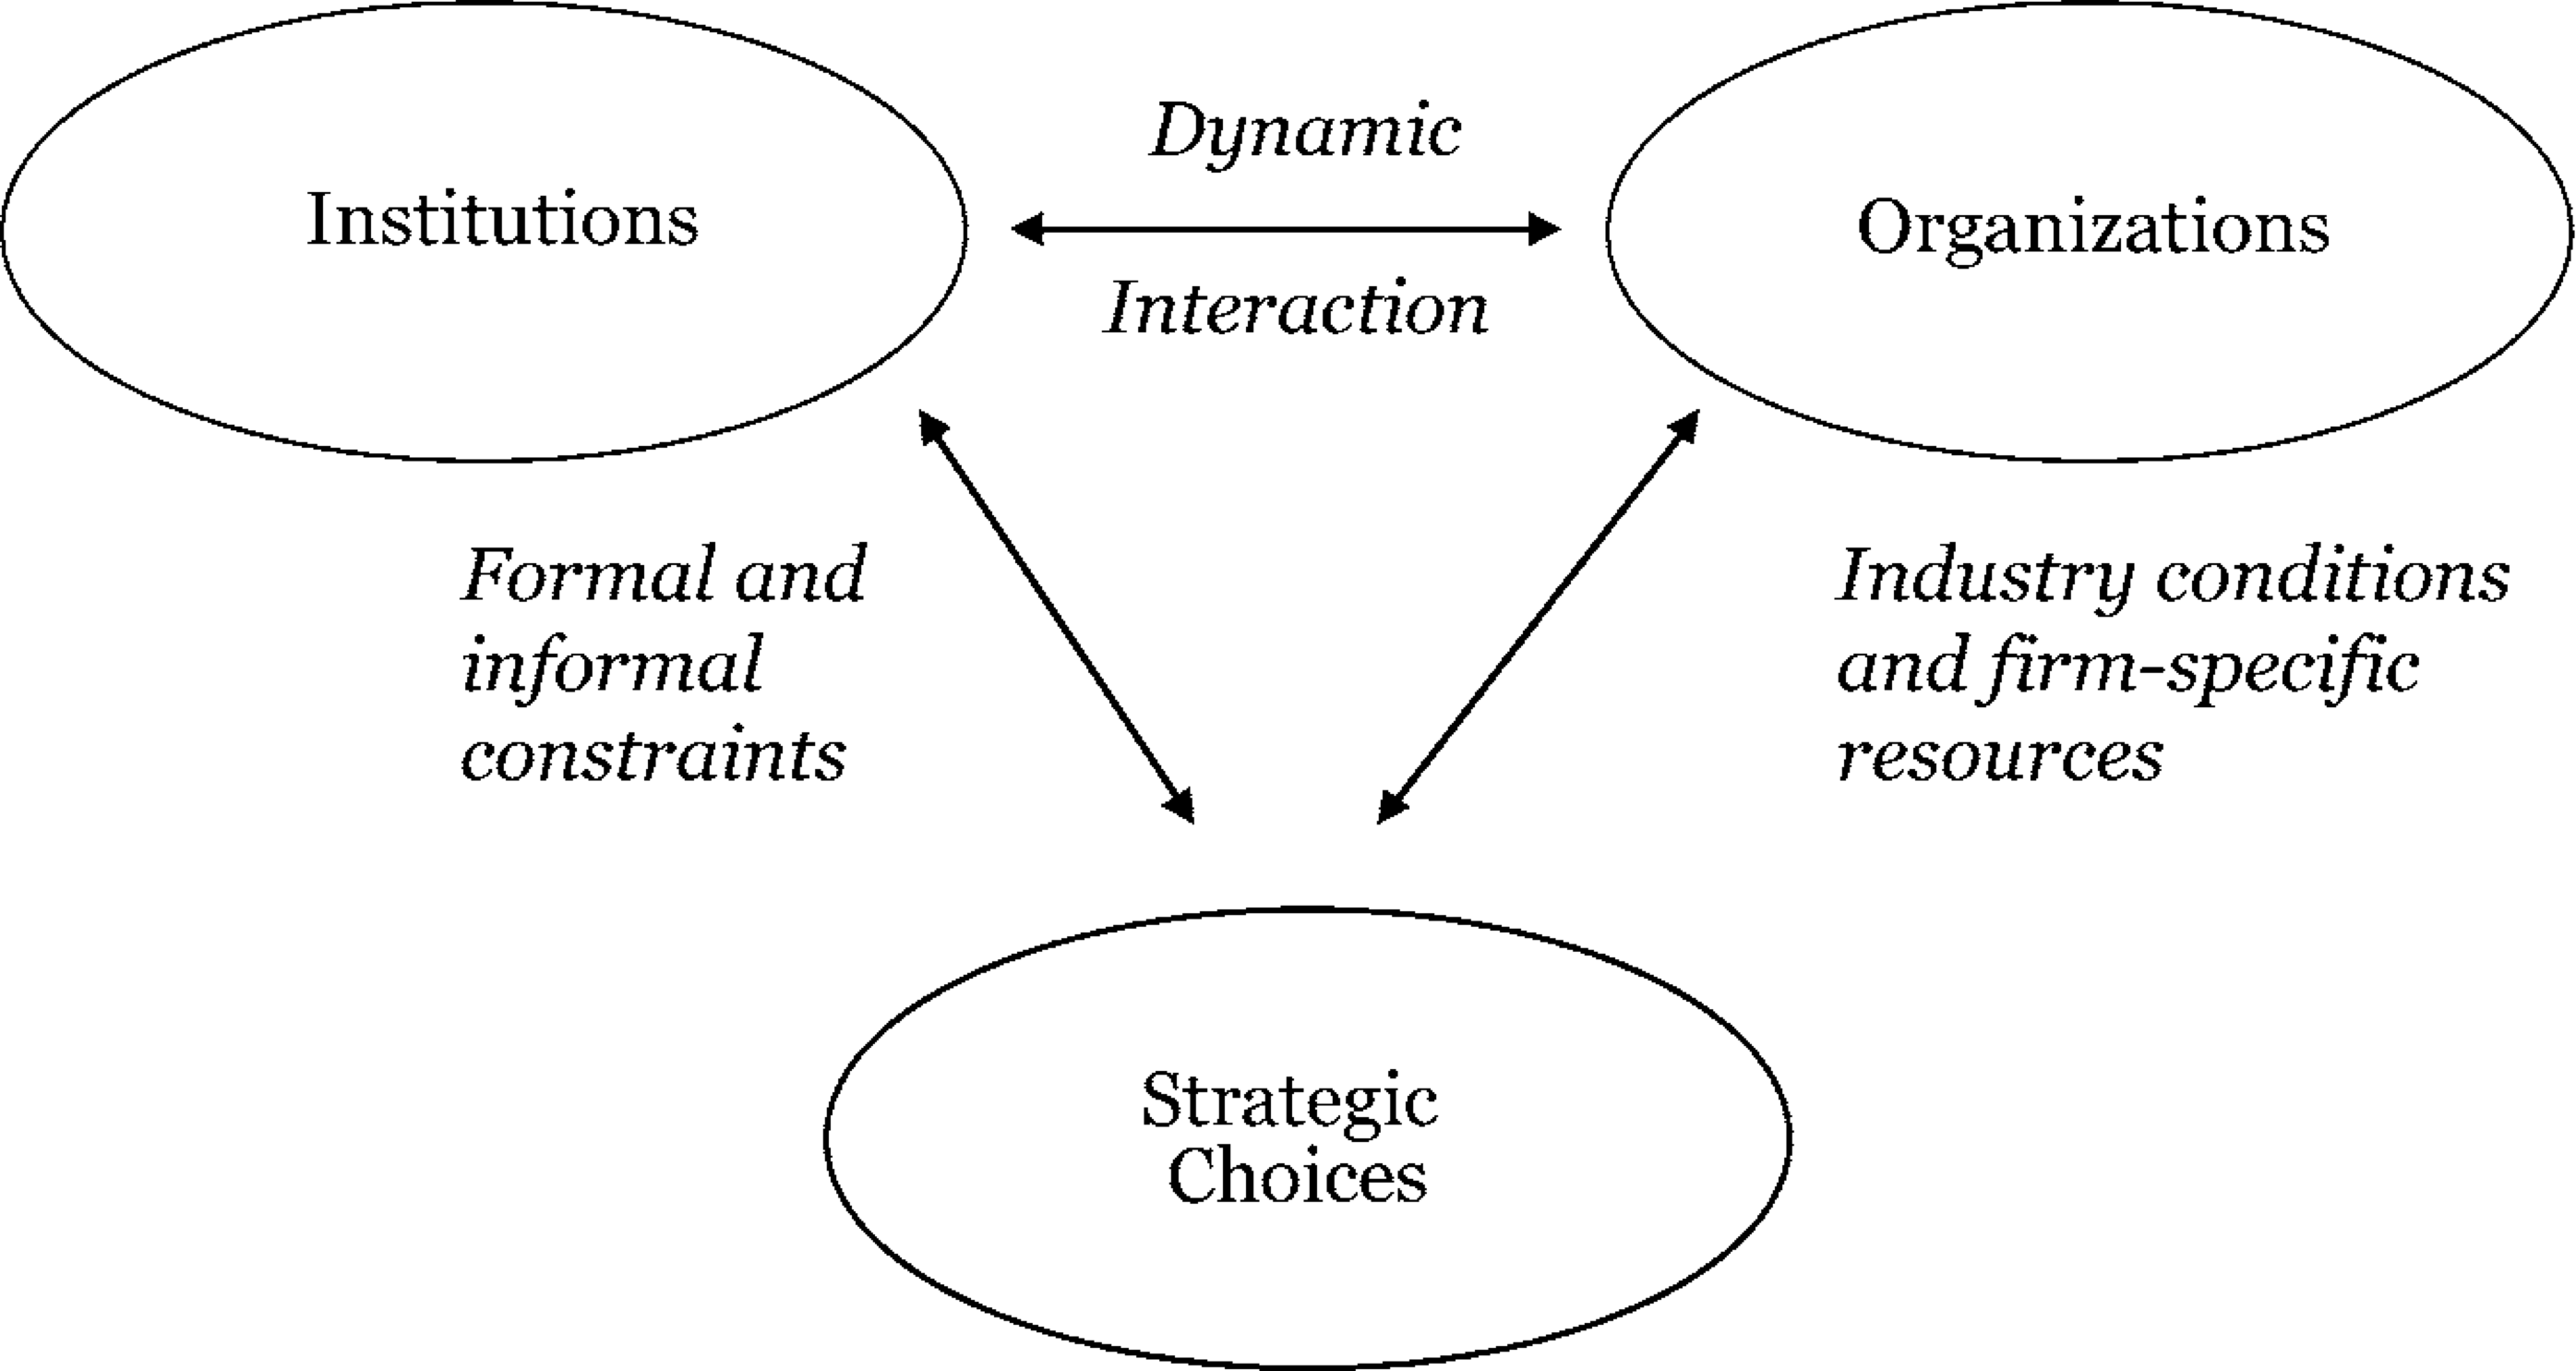
\includegraphics[width=0.65\textwidth]{IBV.pdf}
 	\caption{Institutions, organisations, and strategic choices.
Source: \cite{Peng:2000}}
	\label{fig:ibv}
\end{figure}



Following~\cite{North:1990}, we understand institutions as ``humanly devised constraints
that structure human interaction". Institutional factors function as the formal and
informal ``rules of the game'' that socially constrain contracting practices between the \gls{BoD} and 
executives (\cite{North:1990}).
These formal en informal constraints operate in structures for both social and economic exchanges. 
Institutions are pervasive in that they are capable of shaping the behaviours of multiple actors (i.e. 
individuals, firms, industries, and \glspl{NGO}). More broadly speaking, institutions serve to reduce 
uncertainty for different actors by conditioning the ruling norms of firm behaviours and defining the 
boundaries of what is considered legitimate.~\cite{Peng:2008}\\

So~\ibv~is cannot consist by itself but needs \rbv~\cite{Barney:1991} and \cite{Porter:1980} as is shown in figure~\ref{fig:ibv}. 
Where \rbv looked solely at the firm in a set environment \ibv also takes the surroundings into account. These surroundings are the institutions that govern the environment the \mne is playing the game. 
The actions of institutions can be divided into three pillars. Compliance from the firms occurs through \\(1) expedience (regulative pillar or coercive \iso),\\
 (2) social obligation (normative pillar or normative \iso), or \\
 (3) on a taken for granted basis (cognitive pillar) or mimetic \iso~where organisations respond to uncertainty by adopting patterns of other organisations that are deemed `successful'\cite{Westney:2005,Peng:2008,Kostova:1999,DiMaggio:1983,Scott:1995}.\\ 
\mne conform to these pillars or isomorphisms because these provide legitimacy~\cite{Powell:1991}

Although firms take decisions on the individual resources and capabilities \cite{Barney:1991} the influence of institutions can no longer be ignored. This is the difference between~\rbv and~\ibv. 

According to~\cite{Peng:2003} unfortunately, little is known about how organisations make strategic choices when confronting such large-scale institutional transitions.

\section{Institutional Theory}

 Firms do not only have to look at their resources and capabilities~\cite{Barney:1991}, but have to look at ``the rules of the game''~\cite{Scott:1995}. These so called rules include the environment that the firm \mne~has to adhere to.\\


Not only have   more scholars have come to realise that institutions matter~\cite{Powell:1991,Scott:1995}, and that strategy research cannot just focus on industry conditions and firm resources.\\

The central argument is that “organisations conform to the rules and beliefs systems in the environment because this isomorphism (regulatory, cognitive and normative) earns them legitimacy.

Not only have more scholars have come to realise that institutions matter and, that strategy research cannot just focus on industry conditions and firm resources alone~\cite{Powell:1991,Scott:1995}.

Nowadays institutional theory appears to be a highly insightful approach when probing into organisational strategies in Asia~\cite{Hoskisson:2000}.

\Gls{IB} has long been a favourite topic in academic literature. The term \gls{IB} alone gives over 2M hits in Google Scholar. Since~\cite{Porter:1980} introduced the concept of favourable industries, 

When introduced the \gls{RBV} in international business literature this view gained a lot of support. 
The theory has been expanded upon and \gls{IBV} was introduced by~\cite{Kostova:1999,Meyer:2009,Wang:2012}.


\section{}


%\newacronym{gats}{GATS}{General Agreement on Trade in Services}
\chapter{WTO}

\section{WTO purpose}
The way to view the \wto is not as obvious as one might think on first hand.

\subsection{Negotiating forum}


\subsection{Trade Agreements}
Before the time of the \wto agreements have been reached during the \gls{gats} era. The results of these was a number of agreements regarding the trading of Goods during 1947--1994 trade talk rounds. Not only were agreements reached on trading of goods but also on lower customs duty rates and other trade barriers.

Since the inception of the \wto the new rules have been committed in the \gls{gatt}. The \wto has also been active in settings rules for a number of intellectual property such as copyrights, patents, trademarks, geographical names used to identify products.

\subsection{Set of rules}




\subsection{Dispute Settlement}

When, albeit the negotiated agreements, necessary members can bring disputes before the \wto.
Settling these disputes is the pillar of the \wto trading system. The rules set by the \wto are not as effective when there is no system to enforce these rules. The set of rules is not designed to pass judgement, the priority is to settle disputes (through consultations if possible). 
 
In 2008 only about 136 of the nearly 369 cases had reached the full panel process. Most of the rest have either been notified as settled ``out of court'' or remain in a prolonged consultation phase -- some since 1995 \cite{WTO_History}.

\subsection{}
%\chapter{WTO Roles}

Within the WTO a number of roles can be 


\setcounter{tocdepth}{1}%
\begin{appendices}
%\include{appendices/latex/}
%\include{appendices/latex/}
\end{appendices}


\nocite{*} 
\addcontentsline{toc}{chapter}{Bibliography}
%\bibliography{Thesis_Bib}
\printbibliography%
%\bibliographystyle{apalike} %apalike %h-physrev3 % ducobst
%\input{Thesis_Bib.bib}

\printglossaries%

\end{document}

